\titlepageframe % Specific command 

\begin{tframe}{Motivaci\'on}
	\begin{block}<1->{Tweet mal escrito}
		\begin{center}				
			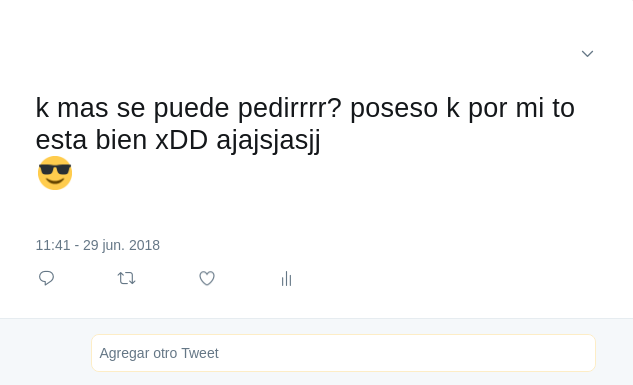
\includegraphics[scale=0.4]{images/TweetBad.png}
		\end{center}
	\end{block}
\end{tframe}

\begin{tframe}{Motivaci\'on (II)}
	\begin{itemize}
		\item Nuevos sistemas de comunicaci\'on (mensajer\'ia instant\'anea, chats, redes sociales, ...)
		\item Uso diferente de los idiomas
		\item Problemas a la hora de analizar textos
		\item<+-> Red social donde predominan: emoticonos, repetici\'on de vocales, uso abusivo de may\'usculas,...
		\item<+-| alert@+> Twitter
	\end{itemize}
\end{tframe}

\begin{tframe}{Motivaci\'on (III): Twitter}
	\begin{itemize}
		\item Ofrece una gran cantidad de datos de libre acceso
		\item Uso de palabras propias de la red social (hashtags, RT, etc.)
		\item<+-> Limitaci\'on de 280 caract\'eres
		\item<+-| alert@+> Abreviaturas, omisi\'on de palabras, abreviaciones, sustituciones fon\'eticas o estructuras no gramaticales
		\item<+-| alert@+> Palabras mal formadas o OOV (\textit{Out-Of-Vocabulary})
	\end{itemize}
\end{tframe}

\begin{tframe}{Objetivos}
	\begin{block}<1->{Objetivo principal}
		Creaci\'on de un corrector que ``normalice'' tweets en espa\~nol.
	\end{block}
	\begin{block}<2->{Subobjetivos}
		\begin{itemize}
			\item Acceso a la API de Twitter para obtener tweets
			\item Tokenizaci\'on de tweets
			\item Detecci\'on entre los tokens las palabras fuera del vocabulario (OOV)
			\item Anotar el tipo de palabra OOV
			\item Correcci\'on de palabras OOV
		\end{itemize}
	\end{block}
\end{tframe}	

\begin{tframe}{Estado del arte}
	\begin{itemize}
		\item Campo de gran inter\'es
		\item Mayor\'ia de trabajos sobre textos en ingl\'es
		\item Introducci\'on al tema de la normalizaci\'on de tweets es el trabajo de Eisenstein, 2013
		\item Normalizaci\'on y adaptaci\'on de herramientas
	\end{itemize}
\end{tframe}

\begin{tframe}{Estado del arte (II): Normalizaci\'on}
	\begin{itemize}
		\item Modelo del canal ruidoso (Shannon 1948), se definen modelo del lenguaje y modelo de error
		\item Brill y Moore (2000) caracterizan el modelo de error
		\item Toutanova y Moore (2002) a\~naden informaci\'on de la pronunciaci\'on
		\item Choudhury et al. (2007) normalizaci\'on SMS usando el modelo de Markov (HMM)
		\item<+-> Cook y Stevenson (2009) expanden el modelo de error 
		\item<+-| alert@+> Pero modelo del canal ruidoso ignora el contexto del OOV
	\end{itemize}	
\end{tframe}

\begin{tframe}{Estado del arte (III): Normalizaci\'on}
	\begin{itemize}
		\item Surgen alternativas que consideran el contexto
		\item Beaufort et al. (2002) m\'etodos de estados finitos combinando las ventajas del modelo del canal ruidoso y el SMS
		\item Kobus et al. (2008) reconocimiento de voz
		\item Aw et al. (2009) traducci\'on autom\'atica estad\'istica (SMT)
		\item<+-> Kaufmann y Kalita (2010) SMT con preprocesado para normalización sint\'actica
		\item<+-| alert@+> Pero todos estos trabajos requieren datos de entrenamiento
	\end{itemize}	
\end{tframe}

\begin{tframe}{Estado del arte (IV): Adaptaci\'on de herramientas}
	\begin{itemize}
		\item En vez de adaptar el texto a las herramientas de an\'alisis
		\item Adaptar las herramientas al texto
		\item Reconocimiento de voz: Gimpel et al. (2011) y Owoputi et al. (2013)
		\item Reconocimiento de entidades: Finin et al. (2010), Ritter et al. (2011) y Liu et al. (2011)
		\item An\'alisis gramatical: Foster et al. (2011)
		\item Modelizaci\'on de di\'alogos: Ritter et al. (2010)
		\item Resumen automático de textos: Sharifi et al. (2010)
		\item Reconocimiento de entidades nombradas (NER): Enron (Minkov, 2005) y CoNLL03 (Tjong, 2003)
		\item NER sobre tweets: Finin et al. (2010)
	\end{itemize}
\end{tframe}

\begin{tframe}{Estado del arte (V): Adaptaci\'on de herramientas}
	\begin{itemize}
		\item Desambiguaci\'on l\'exica o etiquetado gramatical (POST)
		\item Palabras que pueden ser asignadas a m\'as de una clase morfol\'ogica a m\'as de un \textit{part-of-speech} (PoS)
		\item Trabajo más importante y para espa\~nol: SWPoST de S\'anchez-Villamil et al. (2004)
	\end{itemize}
\end{tframe}

\begin{tframe}{Estado del arte (VI): Normalizaci\'on en espa\~nol}
	\begin{itemize}
		\item Tweet-Norm 2013
		\item Dos categorías de candidatos:
			\begin{itemize}
				\item Generaci\'on de candidatos + LM
				\item Transductores o FSTs (\textit{Finite State Transducers})
			\end{itemize}
		\item Mejor participante: Sistema RAE por los autores Gamallo et al. (2013) con un accurancy de 0.781
		\item Sistema basado en FSTs
		\item Otros trabajos: Mosquera et al. (2012) candidatos con indexaci\'on fon\'etica y Olivia et al. (2011)
		\item Sobre mensajes SMS
		\item Tokenizaci\'on en espa\~nol: Gomez-Hidalgo et al. (2013)
	\end{itemize}
\end{tframe}

\begin{tframe}{Estado del arte (VI): Word2Vec}
	\begin{itemize}
		\item Palabras como unidades at\'omicas no hay noci\'on de similaridad entre palabras
		\item Aparecen las representaciones continuas de palabras
		\item Muchos tipos diferentes de modelos: \textit{Latent Semantic Analysis} (LSA) y \textit{Latent Dirichlet Allocation} (LDA)
		\item Distribuciones de palabras aprendidas por redes neuronales.
		\item Las redes neuronales basadad en LM mejoran los modelos N-grama
		\item Dos modelos de redes neuronales destacan basados en LM: \textit{Feed Forward Neural Net Language Model} (NNLM) y \textit{Recurrent Neural Net Language Model} (RNNLM)
		\item<+-> Costosos con grandes candidades de datos
		\item<+-| alert@+> Word2Vec, dos modelos: CBOW y Skip-gram
	\end{itemize}
\end{tframe}

\begin{tframe}{Estado del arte (VII): Word2Vec}
	\begin{itemize}
		\item T\'ecnicas de representaci\'on continua de vectores representan cada palabra como vector distinto
		\item<+-> Se ignora la estructura iterna de las palabras 
		\item<+-| alert@+> Bojanowski et al. (2017) desarrollado por Facebook y denominado fastText
		\item<+-| alert@+> Nuevo enfoque donde cada palabra se representa como una bolsa de caracteres n-gramas.
	\end{itemize}
\end{tframe}

\begin{tframe}{Soluci\'on propuesta}
	\begin{block}<1->{TweetSC (Tweet Spell Checker)}
		Proceso iterativo sobre el tweet a normalizar que se puede dividir en seis fases: tokenizaci\'on, reglas de preproceso, detecci\'on de OOVs, generaci\'on de candidatos para cada OOV, ranking de candidatos y postproceso.
	\end{block}
	\begin{block}<2->{TweetSC. Sistema web}
		Aplicaci\'on web con acceso a la API de Twitter para obtener los tweets mediante consultas introducidas en un formulario de la aplicaci\'on web.
	\end{block}
\end{tframe}

\begin{tframe}{Soluci\'on propuesta (II)}
	\begin{block}<1->{Tokenizaci\'on}
		\begin{itemize}
			\item Primera fase tambi\'en de los analizadores l\'exicos en los compiladores
			\item Genera una lista de tokens que pasan a la siguiente fase
		\end{itemize}
	\end{block}
	\begin{block}<2->{Reglas de preprocesado}
		\begin{itemize}
			\item Se aplican las reglas una a una a los tokens de entrada
			\item Los tokens que acepten alguna regla se eliminan, se crea un OOV anotado como variaci\'on y pasa a la lista final
		\end{itemize}
	\end{block}
	
\end{tframe}

\begin{tframe}{Soluci\'on propuesta (III)}
	\begin{block}<1->{Detecci\'on de OOV}
		\begin{itemize}
			\item Tokens como entrada
			\item Aplicaci\'on de reglas (URL, Hashtag, etc.)
			\item Comparaci\'on con tres diccionarios: espa\~nol, ingl\'es y entidades
			\item Tokens detectados en diccionario espa\~nol se descartan
			\item Tokens detectados en diccionario ingl\'es se anotan como NoEs
			\item Tokens detectados en diccionario de entidades se anotan como Correct
			\item Los tokens no anotados se convierten en OOV y pasan a fase siguiente.
		\end{itemize}
	\end{block}
\end{tframe}

\begin{tframe}{Soluci\'on propuesta (IV)}
	\begin{block}<1->{Generaci\'on de candidatos OOV}
		\begin{itemize}
			\item Primera fase de la correcci\'on
			\item Entrada: lista de OOV
			\item Para cada OOV se genera una lista de candidatos a partir de los m\'etodos:
			\begin{itemize}
				\item LevenshteinFST
				\item Metaphone
				\item L\_L
				\item FastText
				\item Accented
			\end{itemize}
		\end{itemize}
	\end{block}
\end{tframe}

\begin{tframe}{Soluci\'on propuesta (V)}
	\begin{block}<1->{Ranking de candidatos}
		\begin{itemize}
			\item Define la correcci\'on de un candidato o se anota como NoEs si no tiene
			\item Uso de dos marcadores: N-Gram LM y distancia Damerau-Levenshtein
			\item Umbral m\'inimo
		\end{itemize}
	\end{block}
	\begin{block}<2->{Postproceso}
		\begin{itemize}
			\item A\~nadir may\'usculas, exclamaciones, interrogaciones o signos de puntiaci\'on
		\end{itemize}
	\end{block}
\end{tframe}

\begin{tframe}{Implementaci\'on}
	\begin{itemize}
		\item Tres m\'odulos o componentes:
		\begin{itemize}
			\item TweetSCCore
			\item TweetSCExecutable
			\item TweetSCWeb
		\end{itemize}
		\item Java + Python
		\item Google Cloud Engine
		\item Sistema din\'amico para que se puedan a\~nadir nuevos m\'etodos y eliminar otros de forma sencilla
		\item Dos m\'etodos de normalizaci\'on:
		\begin{itemize}
			\item DictionaryMethod
			\item TweetSCMethod
		\end{itemize}
		\item Aplicaci\'on web: \url{https://jmorenov.github.io/TweetSC/}
	\end{itemize}
\end{tframe}

\begin{tframe}{Arquitectura del sistema}
	\begin{center}
		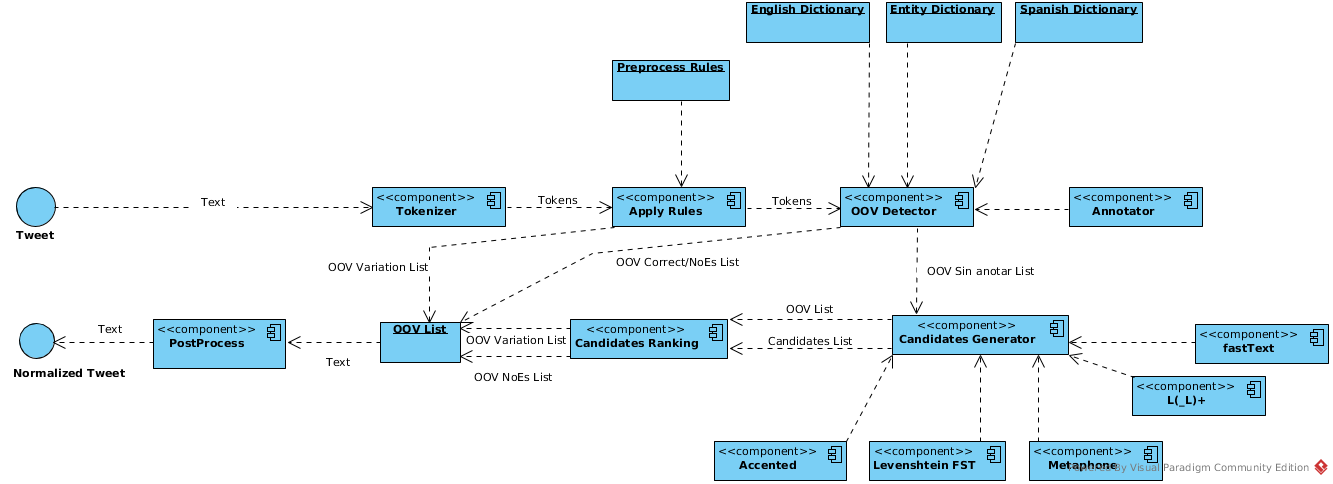
\includegraphics[scale=0.35]{images/DiagramaDelSistema}
	\end{center}
\end{tframe}

\begin{tframe}{Evaluaci\'on}
	\begin{block}<1->{Metodolog\'ia}
		\begin{itemize}
			\item Tarea compartida Tweet-Norm 2013
			\item Medida de evaluaci\'on: correcci\'on de errores
		\end{itemize}
	\end{block}
	\begin{block}<2->{Corpus}
		\begin{itemize}
			\item Tweet-Norm 2013
			\item Dos subconjuntos de tweets
			\item Desarrollo (500 tweets) y evaluaci\'on (600 tweets)
		\end{itemize}
	\end{block}
	\begin{block}<3->{Gold standard}
		Sistema Rae con un resultado de 0.781
	\end{block}
\end{tframe}

\begin{tframe}{Evaluaci\'on (II)}
	\begin{block}<1->{Experimentos}
	\begin{adjustbox}{max width=\textwidth}
		\begin{tabular}{|c|c|c|c|c|c|c|}
\hline 
\textbf{M\'etodo} & \textbf{N} & \textbf{Positivos} & \textbf{Negativos} & \textbf{Errores} & \textbf{\textit{Accurancy (\%)}} & \textbf{Tiempo(s)} \\ 
\hline 
DictionaryM & 10 & 6 & 10 & 4 & 31.578 & 1.889 \\ 
\hline 
DictionaryM & 100 & 18 & 82 & 39 & 15.652 & 7.705 \\ 
\hline 
DictionaryM & 500 & 131 & 405 & 162 & 21.510 & 18.926 \\ 
\hline 
TweetSCM & 10 & 11 & 5 & 4 & 57.894 & 4.502 \\ 
\hline 
TweetSCM & 100 & 23 & 77 & 39 & 20.0 & 45.118 \\ 
\hline 
TweetSCM & 500 & 122 & 423 & 160 & 20.032 & 227.438 \\ 
\hline 
Sistema RAE & - & - & - & - & 78.1 & - \\ 
\hline 
\end{tabular}
\end{adjustbox}
	\end{block}
\end{tframe}

\begin{tframe}{Conclusiones}
	\begin{itemize}
		\item Dise\~nado e implementado un corrector de texto en espa\~nol para Twitter
		\item Componente de investigaci\'on
		\item M\'as all\'a del estado del arte en algunos aspectos: Word2Vec, FST Levenshtein, algoritmo del met\'afono y LM N-grama
		\item Desarrollados tres modulos: TweetSCCore, TweetSCExecutable, TweetSCWeb
		\item Resultados de los experimentos modestos
		\item Proyecci\'on para mejorar estos resultados
	\end{itemize}
\end{tframe}

\begin{tframe}{Conclusiones (II)}
	\begin{center}
		\highlightbf{?`Preguntas?}
	\end{center}
\end{tframe}